\documentclass[compress, containsverbatim,mathserif, xcolor=dvipsnames, unicode]{beamer}


%tema
\usetheme{Antibes}
%\usecolortheme[named=Maroon]{structure}
\usecolortheme{beaver}
\setbeamercolor{titlelike}{fg=black, bg=purple}
\setbeamercolor{palette primary}{fg=pink, bg=purple}
\setbeamercolor{palette secondary}{fg=purple, bg=pink}
\setbeamercolor{palette tertiary}{bg=purple, fg=black}
\setbeamercolor{palette quaternary}{bg=purple, fg=black}
\setbeamercolor{frametitle}{bg=purple}
\setbeamercolor{block body}{bg=pink, fg=black}
\setbeamercolor{block title}{bg=purple, fg=white}
\setbeamertemplate{itemize item}{\color{purple}$\blacksquare$}
\setbeamertemplate{itemize subitem}{\color{purple}$\blacksquare$}
\setbeamercolor{item projected}{bg=purple,fg=white}
\setbeamercolor{section in toc}{fg=purple,bg=white}





% zbog srpskog
\usepackage[serbian]{babel}
\usepackage[utf8]{inputenc}
\usepackage[T2A]{fontenc}

% za matematiku
\usepackage{amsmath}
\usepackage{amssymb}
\usepackage{fontawesome5}

\usepackage{xcolor}

\newtheorem{primer}{Primer}[section]

\title{Optimizacije kroz GCC, LLVM i Native Image}
\author{Tamara Stojković, Emilija Stošić, Teodora Isailović}
\institute{Metodologija stručnog i naučnog rada \\ Matematički fakultet \\ Univerzitet u Beogradu}
\date{
	\footnotesize{Beograd, decembar 2022.}	
}

\begin{document}

\begin{frame}
\titlepage

\begin{figure}[h!]
    \centering
    \begin{flushleft}
    
\includegraphics[width=15mm]{logo.png}
    \end{flushleft}
\end{figure}
\end{frame}

\begin{frame}{Sadržaj}
\tableofcontents
\end{frame}

\section{Uvod}
\begin{frame}{Uvod}
\vspace{\baselineskip}
\begin{itemize}
	\item Optimizacija - tehnika transformacije dela programa, sa ciljem poboljšanja performansi koda
    \item Oblast u kojoj se danas vrši većina istraživanja kompajlera
    \item Kompajleri - različiti nivoi optimizacije
	\item Na nivoima kompromisi između mera - kvalitet koda, veličina koda, vreme kompilacije
    \item Izbor kompajlera i nivoa optimizacije zavise od konkretnog programa
\end{itemize}
\end{frame}



\section{Osnovna podela optimizacija}
\subsection{Optimizacije međukoda}
\begin{frame}{Lokalne optimizacije}
    
    \begin{itemize}
        \item Razlikujemo: lokalne, globalne i međuproceduralne
        \item  \textcolor{purple}{Lokalne optimizacije} služe za ubrzavanje malih delova neke funkcije, najlakše za izvođenje
        \item Tehnike lokalne optimizacije koje razlikujemo: 
                \begin{itemize}
                    \item Eliminacija čestih podizraza
                    \item Slaganje konstanti
                    \item Propagacija kopija
                    \item Smanjenje snage operatora
                    \item Eliminacija mrtvog koda
                    \item Algebarsko pojednostavljenje i reasocijacija
                    \item Kompozicija lokalnih transformacija
                \end{itemize}
        \end{itemize}
\end{frame}


\begin{frame}{Globalne i međuproceduralne optimizacije}
    \begin{itemize}
        \item \textcolor{purple}{Globalne optimizacije} primenjuju se na jednu po jednu funkciju, slične lokalnim
        \item Globalne optimizacije koje razlikujemo: 
                \begin{itemize}
                    \item Globalna eliminacija mrtvog koda
                    \item Globalno propagiranje konstanti
                    \item Globalna eliminacija čestih podizraza
                    \item Optimizacija kretanje koda
                    \item Pomeranje invarijantog koda
                    \item Parcijalna eliminacija suvišnosti
                \end{itemize}
        \item \textcolor{purple}{Međuproceduralna optimizacija } - radi na celokupnom grafu kontrole toka
        \item Vrši se na nivou celog programa tj. više funkcija 
        \item Najpoznatija tehnika je uvlačenje definicija funkcija 
        \end{itemize}
\end{frame}


\subsection{Optimizacije koda}
\begin{frame}{Optimizacije koda}
    
    \begin{itemize}
        \item Optimizovani međukod se prevodi u asemblerski tj. mašinski kod - faza generisanja
        \item  Bitne su specifične karakteristike mašine
        \item Razlikujemo  sledeće tehnike: 
                \begin{itemize}
                    \item Optimizacija redosleda instrukcija - obuhvata fazu odabira instrukcija, alokacije registara i raspoređivanja instrukcija
                    \item Optimizacija upotrebom keša - zasniva se na prostornoj i vremenskoj lokalnosti, cilj da bude što bolja
                \end{itemize}
        \end{itemize}
\end{frame}

\section{Napredne optimizacije u okviru kompajlera GCC/LLVM}
\subsection{Optimizacije u okviru kompajlera GCC}
\begin{frame}{Optimizacije u okviru kompajlera GCC}
    \begin{itemize}
        \item Opcije koje su vrlo značajne u procesu kompilacije, su opcije za optimizaciju
        \item Nivo optimizacije koju kompajler vrši se kontroliše
opcijom -On, gde je n nivo zahtevane optimizacije
        \item Postoji sedam nivoa optimizacije : -O0, -O1, -O2, -O3, -Os, -Og, -Ofast
    \end{itemize}
     \begin{figure}[h!]
        \begin{center}
       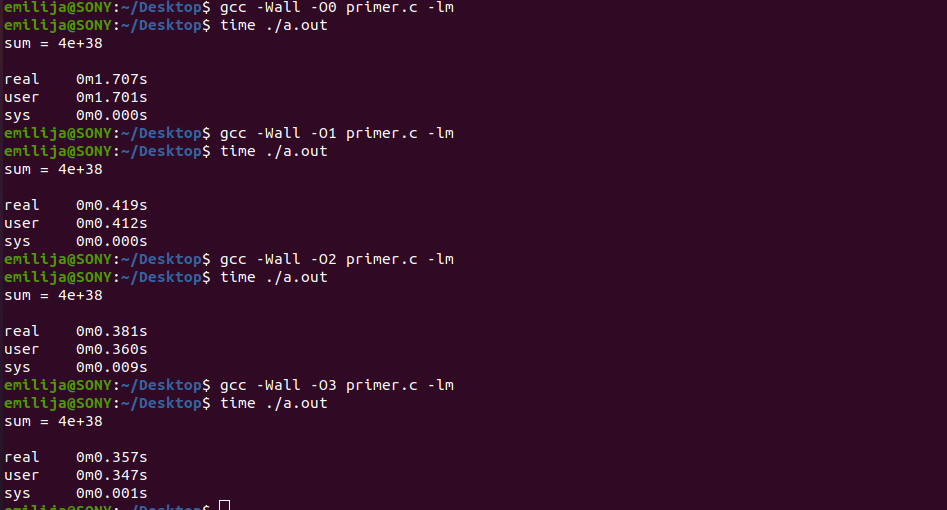
\includegraphics[scale = 0.3]{../pics/test.png}
       \end{center}
       \caption{Rezultati optimizacije kod GCC kompajlera}
    \end{figure}    
\end{frame}

\subsection{Optimizacije u okviru kompajlera LLVM}
\begin{frame}{Optimizacije u okviru kompajlera LLVM}
    \begin{itemize}
        \item Optimizacije u vidu prolaza
        \item Svi LLVM prolazi su podklase klase Pass
        \item Funkcionalnosti su implementirane tako što prevazilaze virtuelne metode nasleđene od klase Pass
        \item Analysis Passes prikuplja informacija koje 
služe za otklanjanje grešaka ili vizuelizaciju programa
        \item Transform Passes se koriste za optimizaciju koda
        \item Utility Passes služe za dobijanje raznih
informacija, koje su bitne za razvoj drugih prolaza
    \end{itemize}    
\end{frame}


\begin{frame}{Optimizacije u okviru kompajlera LLVM}
    \begin{itemize}
        \item Postoji sedam nivoa optimizacije : -O0, -O1, -O2, -O3, -O4, -Os, -Oz
        \begin{figure}[h!]
        \begin{center}
          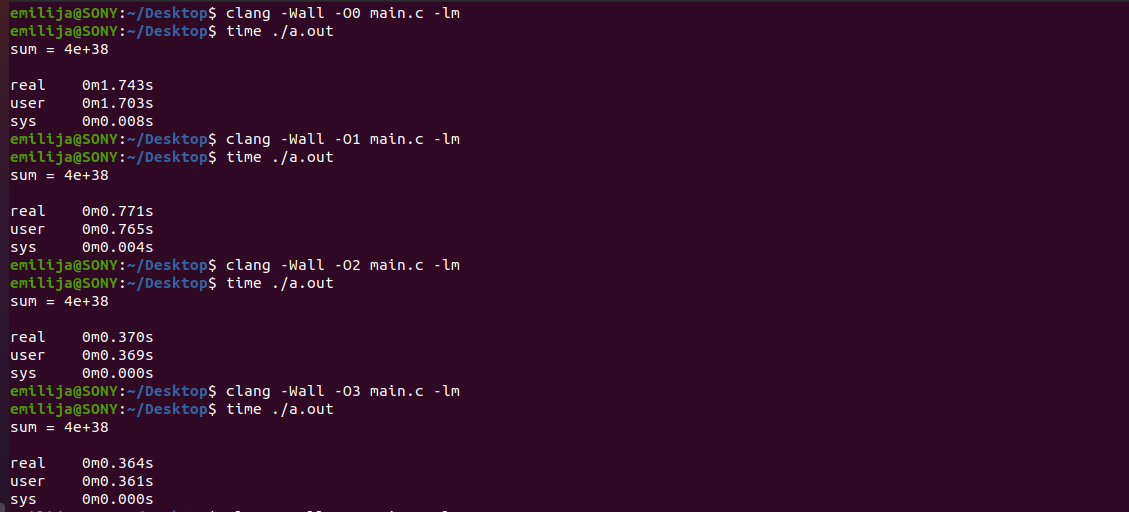
\includegraphics[scale = 0.25]{../pics/test2.png}
        \end{center}
       \caption{Rezultati optimizacije kod LLVM kompajlera}
    \end{figure} 
    \end{itemize}    
\end{frame}

%\section{Native Image}
%\begin{frame}{Native Image}
%\vspace{\baselineskip}
%\begin{itemize}
%	\item Ahead-Of-Time kompilacija
%    \item Od bytecode-a do izvršivog koda (native image) određene platforme
%    \item Rezultat je statički povezan kod koji se izvršava direktno na procesoru 
%    \item Podržava jezike kao što su Java, Scala, Kotlin itd.
%	\item Najpoznatiji primeri Native Image iz GraalVM i Ngen za .NET Framework-a
%\end{itemize}
%\end{frame}
%
%\subsection{Problemi i optimizacije}
%\begin{frame}{Problemi i optimizacije - Native Image}
%    \begin{itemize}
%        \item Statička analiza (Closed World Assumption)
%        \item Za nerazrešene delove potreban konfiguracioni fajl \\ (tracing agent)
%        \item Rezultujući kod se izvršava brže i zahteva manje memorije u odnosu na JVM
%        \item 
%    \end{itemize}
%        
%\end{frame}

\section{Native Image}
\subsection{Pojam}
\begin{frame}{Native Image - pojam}
    \begin{itemize}
        \item Od bytecode-a do izvršivog koda (native image) određene platforme
        \item Ahead-Of-Time kompilacija
        \item Rezultujući kod se izvršava brže i zahteva manje memorije u odnosu na VM
        \item Najpoznatiji primeri Native Image iz GraalVM i Ngen (CrossGen) za .NET Framework (Core)            
    \end{itemize} 
    \vspace{1em}
    \begin{figure}[h!]
        \begin{center}
            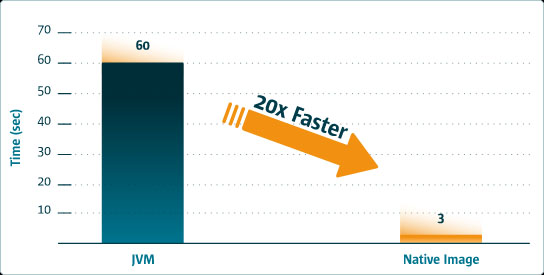
\includegraphics[scale = 0.25]{../pics/alibaba_pic.jpg}
        \end{center}
        \caption{Ubrzanje native image-a u odnosu na JVM}
    \end{figure} 
\end{frame}

\subsection{Prevodjenje}
\begin{frame}{Prevodjenje}
    \begin{itemize}
        \item Statička analiza (Closed World Assumption)
        \vspace{1em}
        \item Problemi i optimizacije:
        \begin{itemize}
            \item Reflection API
            \item Dynamic proxy
            \item Java Native Interface
        \end{itemize}        
        \vspace{1em}
        \item Za nerazrešene delove potreban konfiguracioni fajl \\ (tracing agent)
        \item Fallback image
    \end{itemize}
\end{frame}

\section{Literatura}
\begin{frame}{Literatura}
    \begin{itemize}
        % \item Compiler Design - Code Optimization
        \item Kompajleri Stanford \\ \scriptsize \url{https://web.stanford.edu/class/archive/cs/cs143/cs143.1128/}  \normalsize
        \item The Dragon Book Compilers: Principles, Techniques (Alfred V. Aho, Monica S. Lam, Ravi Sethi, and Jeffrey D. Ullman) \normalsize
        \item Options That Control Optimization \\ \scriptsize \url{https://gcc.gnu.org/onlinedocs/gcc/Optimize-Options.html} \normalsize
        \item LLVM's Analysis and Transform Passes \\ \scriptsize \url{https://llvm.org/docs/Passes.html} \normalsize
        \item GraalVM Manual - Native Image \\ \scriptsize \url{https://www.graalvm.org/22.0/reference-manual/native-image/} \normalsize
    \end{itemize}
\end{frame}

\end{document}

    
